\chapter{Results}\label{chapter:results}
In this chapter, we present the results of our experiments.
First, the properties of the generated dataset are presented and visualized.
Then, the results of the different retrieval methods are presented and compared.
Finally, the results of ranking the LLM answers are presented and the influence of the different prompting strategies, model sizes, pre training methods and question types are discussed.

\section{Dataset}
Our dataset is constructed according to the procedure described in section \ref{sec:dataset}.
We now go more in depth on the properties of the final dataset, considering the type of queries, the number of answers per query and the length of the answers.
\\
The total number of queries in the final dataset is 50, each of which is accompanied by between 39 and 249 answers.
The number of answers depends on how many of the given answer in the base dataset by \cite{goeuriot:2021} were, still available, i.e. not from Reddit or Twitter.
Since this was not the same for all queries, the number of answers per query varies.
On average, there are about 178 evaluated documents per query available.

\subsection{Queries}
We identify two different query types in the dataset: questions and keyword queries.
Questions are queries that are formulated as a question, e.g. ``Is a ketogenic diet suitable for people with diabetes?'', while keyword based queries are more in the style of search engine queries, e.g. ``keto diet diabetes''.
\begin{table}[tb]
\centering
\begin{tabularx}{\textwidth}{XX}
\hline
\textbf{Keyword-Based Queries} & \textbf{Question-Type Queries} \\
\hline
best apps daily activity exercise diabetes & What are the most common chronic diseases? \\
\hline
my risk for developing type 2 diabetes & Is a ketogenic / keto diet suitable for people with diabetes? \\
\hline
multiple sclerosis stages phases & Can diabetes be cured? \\
\hline
\end{tabularx}
\caption{Samples of Keyword vs Question Type Queries}
\label{table:querie-samples}
\end{table}
Table \ref{table:querie-samples} shows some examples of the two query types.
Query topics are diverse, ranging from general queries about chronic diseases to specific questions about the suitability of certain diets for people with diabetes.
\\\\
\begin{figure}
\centering
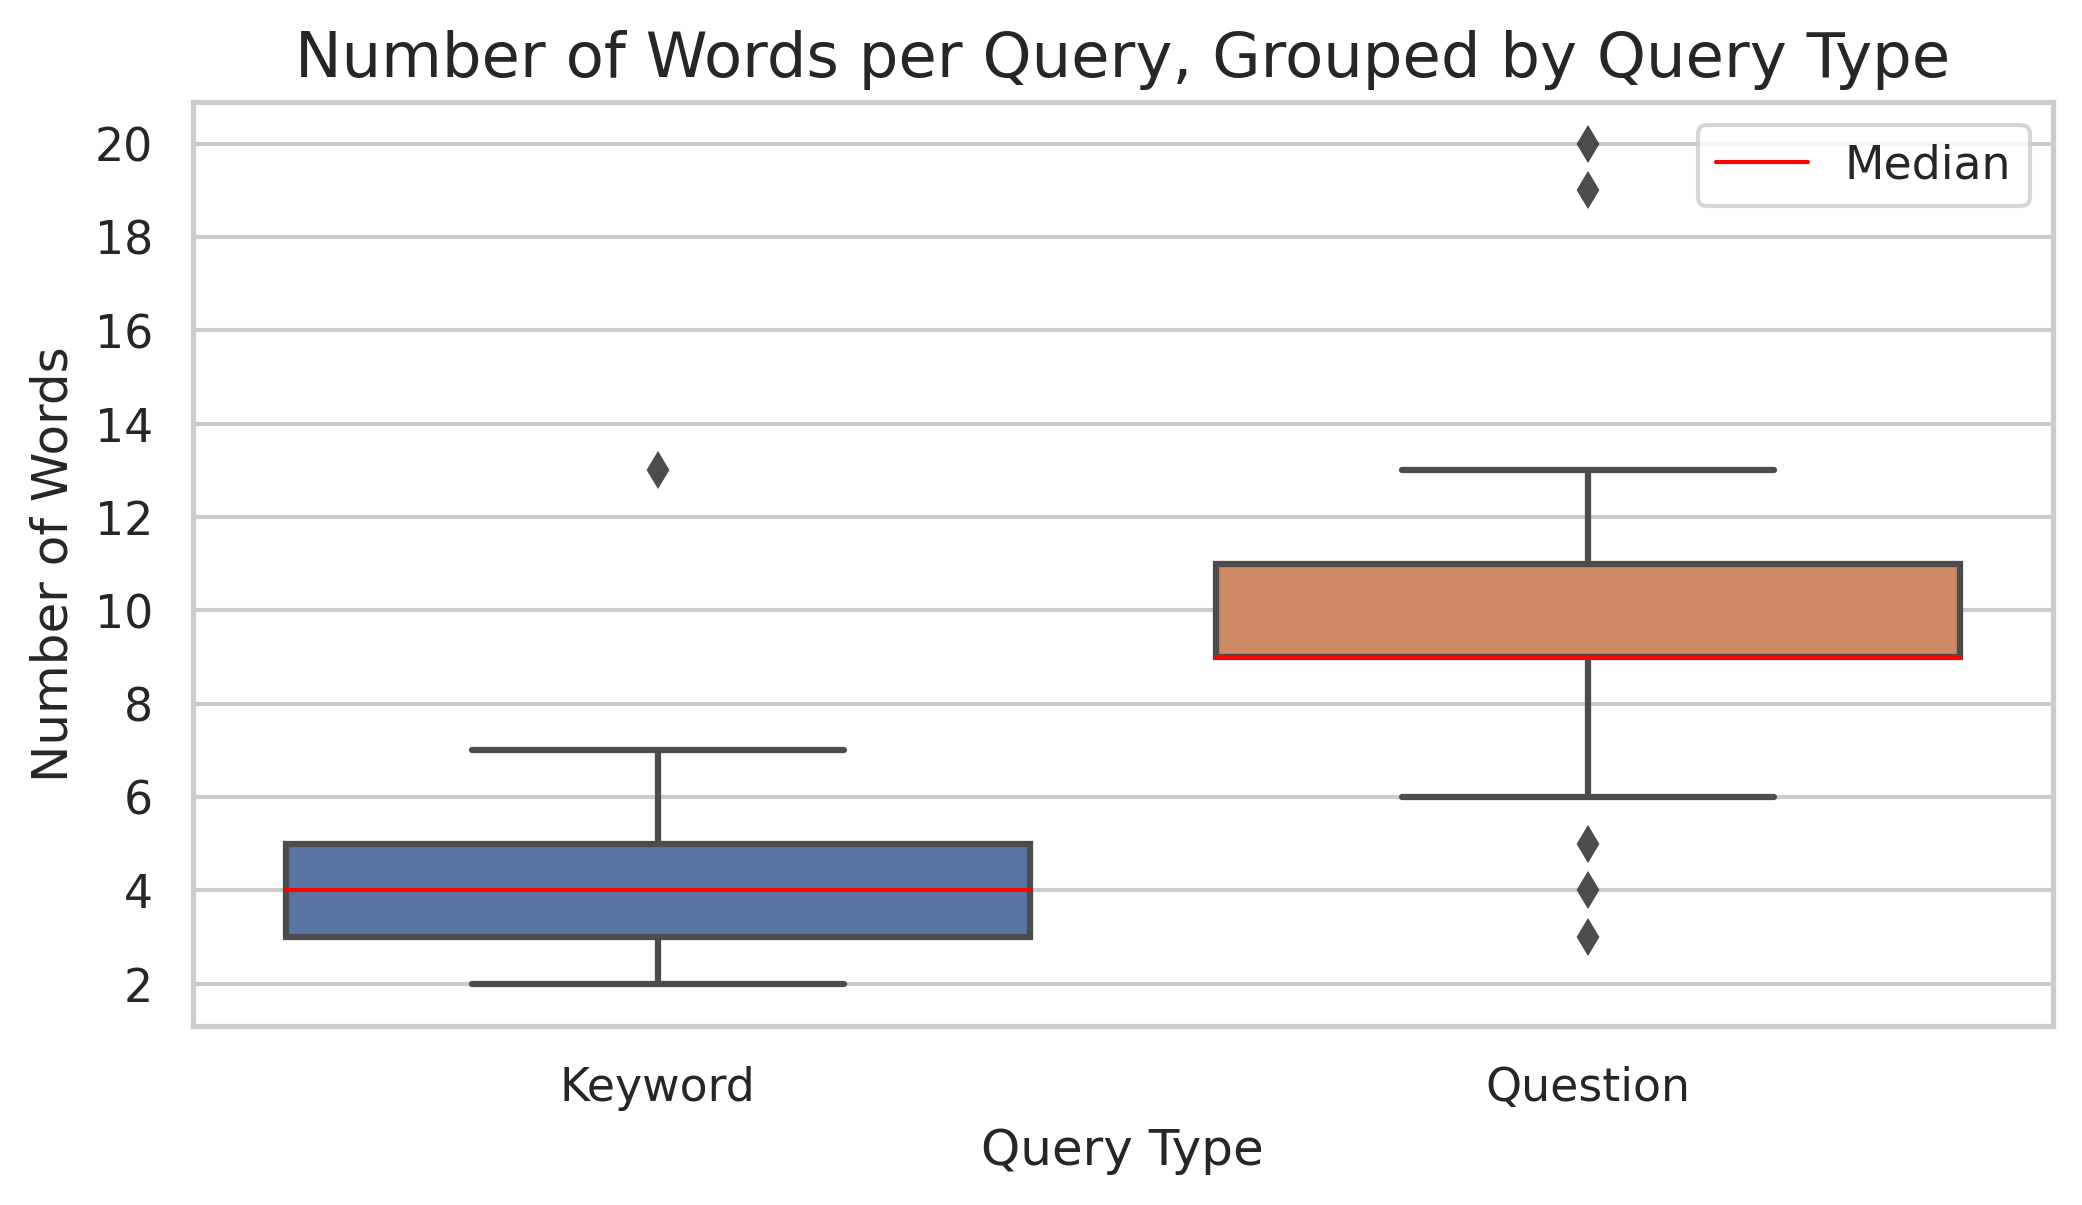
\includegraphics[width=\textwidth]{images/num_words_per_query.png}
\caption{Boxplot of the number of words per query, split by query type. Keyword queries are shorter than question queries with a median of 4 words compared to 7 words for the question queries.}
\label{fig:num_words_per_query}
\end{figure}
In total, we identify 17 question-style queries and 33 keyword-style queries.
Figure \ref{fig:num_words_per_query} shows the number of words per query for both query types.
As expected, the keyword queries are shorter than the question queries, with a median of 4 words compared to 7 words for the question queries.
The shortest query is only two words long, while the longest query is 20 words long.
\subsection{Documents}
\begin{table}[tb]
\centering
\begin{tabular}{ll}
\hline
\textbf{Domain} & \textbf{Occurrences} \\
\hline
www.healthline.com & 603 \\
www.nationalmssociety.org & 419 \\
www.ms.org.au & 198 \\
jhu.pure.elsevier.com & 191 \\
www.msif.org & 183 \\
www.psychologytoday.com & 161 \\
www.urotoday.com & 155 \\
www.news-medical.net & 150 \\
www.sleepfoundation.org & 141 \\
www.aafp.org & 139 \\
\hline
\end{tabular}
\caption{Top 10 Most Frequently Occurring Domains}
\label{tab:top_domains}
\end{table}
The documents in the dataset are scraped from a total of 234 different domains.
Table \ref{tab:top_domains} shows the top 10 most frequently occurring domains in the dataset.
Most domains are health related, belonging to either health organizations, medical journals or health news websites.
Some domains are more general, e.g. there are also wikipedia.org pages in the dataset, as well as some domains from essay writing or homework help websites.
A total of 133 domains show up less than 10 times in the dataset, while 44 domains show up only once.
\\\\
\begin{figure}[tb]
\centering
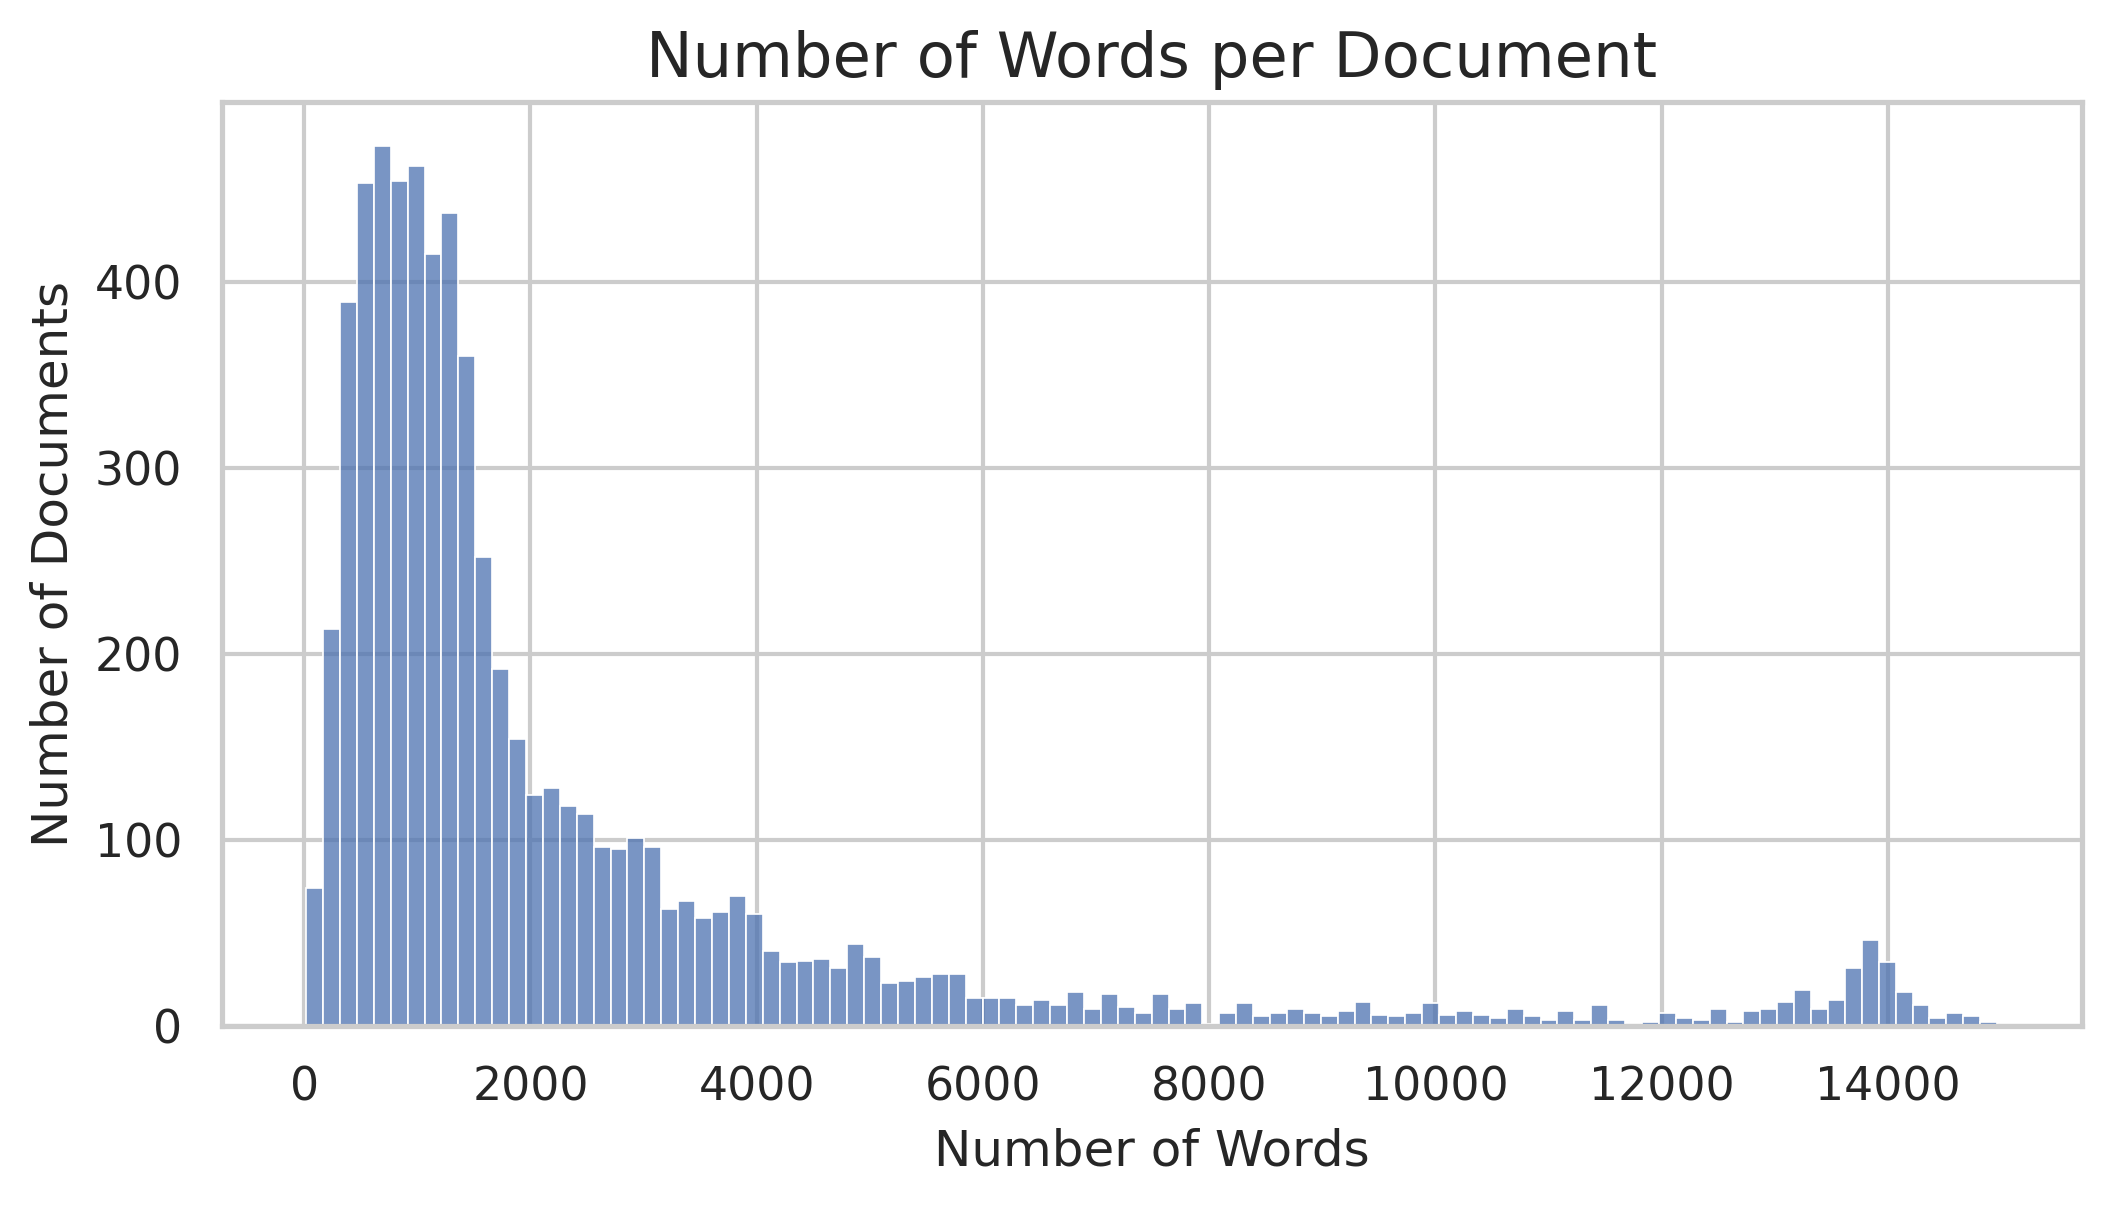
\includegraphics[width=\textwidth]{images/num_words_per_passage.png}
\caption{Histogram of the number of words per document. The plot is cut at 15 000 words, which excludes 120 or 2\% of the documents. The median number of words per document is 1354, while the mean is 2901.}
\label{fig:num_words_per_document}
\end{figure}
After preprocessing, the documents are cleaned of all HTML tags and of HTML elements containing fewer than 50 characters.
Figure \ref{fig:num_words_per_document} shows that the number of words per document is very high, with a median of 1354 words and a mean of 2901 words.
This is natural for documents scraped from the web, which do not only contain the main text, but also navigation bars, footers, sidebars and other elements.
Those can not be fully removed with our trivial preprocessing methods.
\subsection{Document Metrics}
The document metrics in the dimensions of readability, credibility and relevance are based on the human annotations from \cite{goeuriot:2021}.
In general, a surprisingly high number of documents are rated as not relevant to the given query.


\section{Retrieval Pipelines}

\section{Ranking of Generated Answers}